\section{Results}
\label{sec:results}

\para{Main benchmark results.} \Tabref{tab:main_results} compares direct LLM judgment, the grouped stylometric baseline, and the grouped embedding probe on the controlled six-mode corpus. \gptfourone reaches perfect accuracy and macro-F1, while the stylometric baseline reaches 0.400 accuracy and the embedding probe reaches 0.489. The paired bootstrap gap between the LLM judge and the stylometric baseline is +0.602 accuracy (95\% CI: [0.555, 0.650]) and +0.618 macro-F1 (95\% CI: [0.573, 0.665]).

\begin{table}[t]
    \centering
    \caption{Controlled six-mode classification results. Higher is better for all metrics. Best results are in \textbf{bold}.}
    \label{tab:main_results}
    \begin{tabular}{@{}lcc@{}}
        \toprule
        Method & Accuracy & Macro-F1 \\
        \midrule
        \gptfourone zero-shot judge & \textbf{1.000} & \textbf{1.000} \\
        Stylometric baseline & 0.400 & 0.386 \\
        Embedding probe & 0.489 & 0.477 \\
        \bottomrule
    \end{tabular}
\end{table}


\begin{figure}[t]
    \centering
    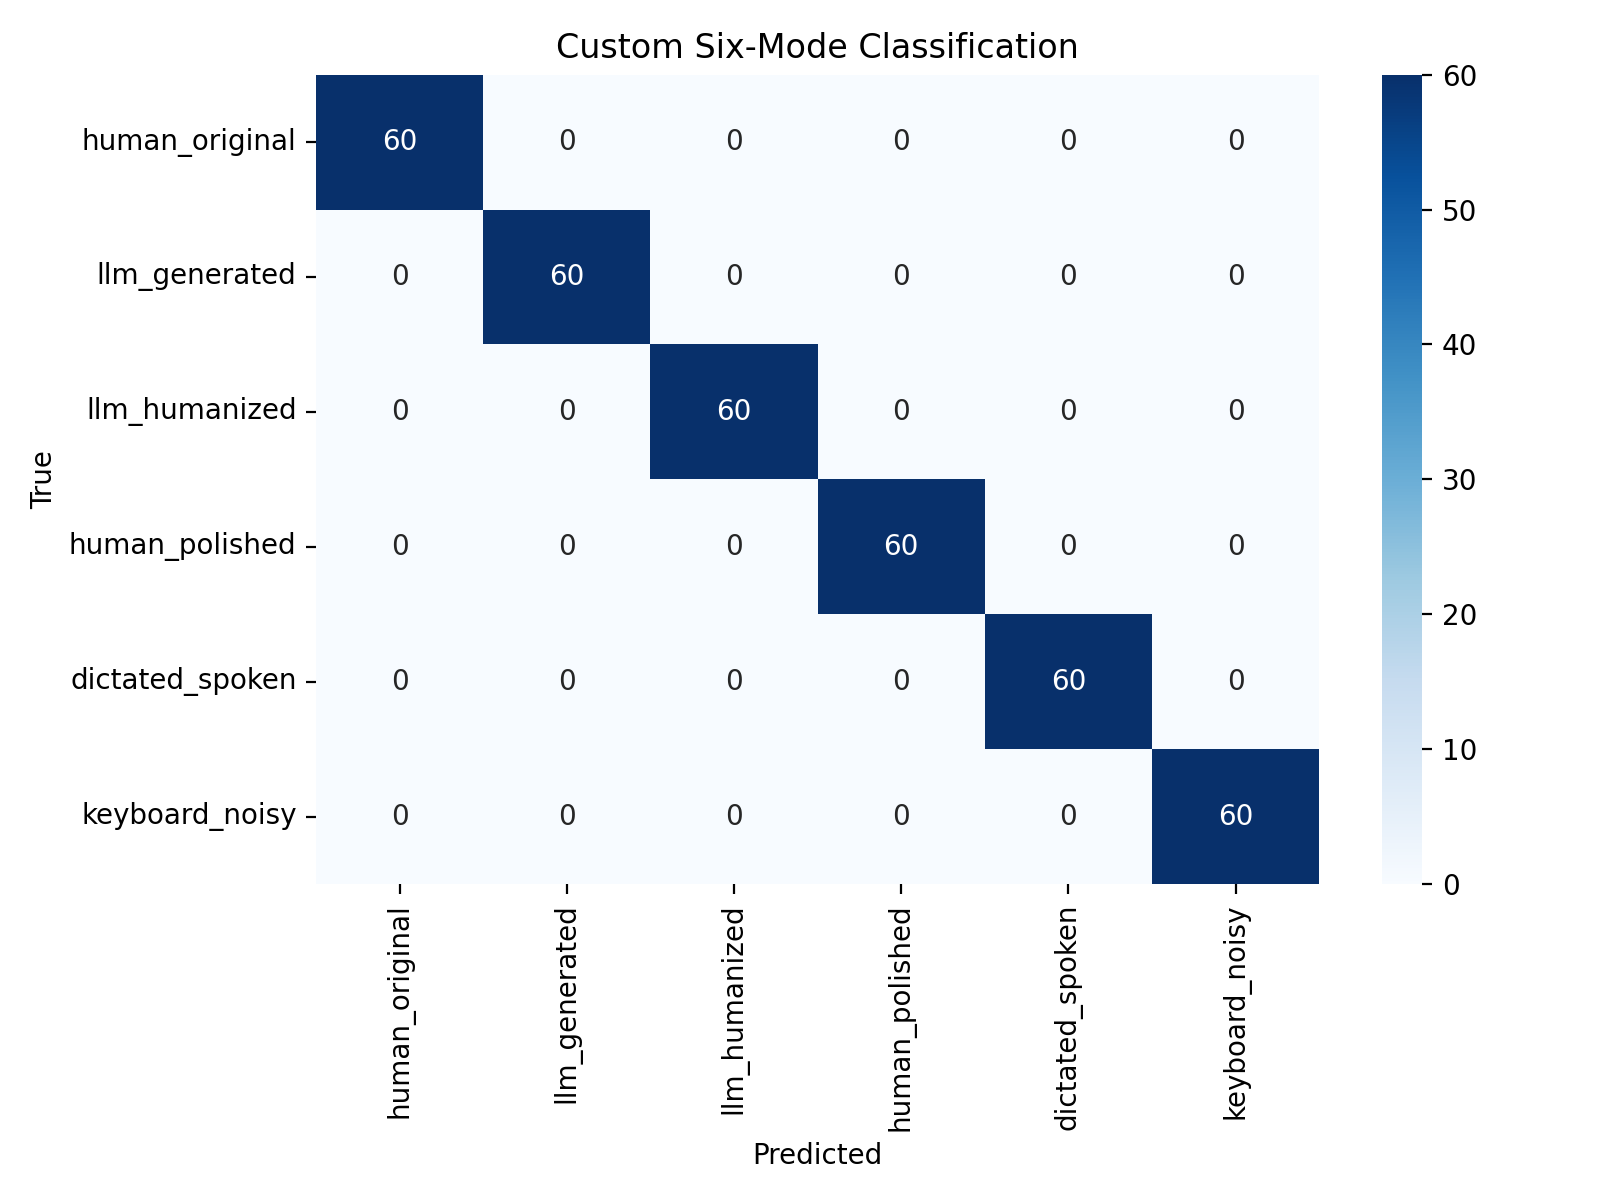
\includegraphics[width=0.78\linewidth]{figures/custom_mode_confusion.png}
    \caption{Confusion matrix for zero-shot six-way mode classification on the controlled corpus. The matrix is perfectly diagonal, but the underlying probability outputs are not saturated: representative correct-class probabilities range from 0.75 to 0.94.}
    \label{fig:custom_confusion}
\end{figure}

\para{The task is easy, but not vacuous.} \Figref{fig:custom_confusion} shows a perfectly diagonal confusion matrix for the controlled benchmark. The model does not appear to solve the task only by assigning near-certain probabilities to every example: representative correct-class probabilities remain moderate, including 0.75 for \texttt{human\_polished}, 0.78 for \texttt{dictated\_spoken}, and 0.80 for \texttt{llm\_humanized}. That pattern is consistent with a highly separable task rather than a degenerate prompt that simply elicits one fixed label.

\para{Embedding probes recover mode above chance.} The grouped embedding probe reaches 0.489 accuracy on unseen content anchors, well above the 0.167 chance rate. A corrected 20-run permutation test yields shuffled accuracies between 0.139 and 0.203 and an observed $p=0.0476$. \Tabref{tab:probe_recall} shows that the probe separates overt mode shifts most clearly: \texttt{dictated\_spoken} reaches 0.700 recall, while the subtler \texttt{human\_original} and \texttt{human\_polished} classes remain much harder.

\begin{table}[t]
    \centering
    \caption{Per-class recall for the grouped embedding probe on unseen content anchors. Overt production shifts are easiest to recover from embeddings alone.}
    \label{tab:probe_recall}
    \begin{tabular}{@{}lc@{}}
        \toprule
        Mode & Recall \\
        \midrule
        \texttt{dictated\_spoken} & \textbf{0.700} \\
        \texttt{llm\_generated} & 0.617 \\
        \texttt{keyboard\_noisy} & 0.567 \\
        \texttt{llm\_humanized} & 0.567 \\
        \texttt{human\_original} & 0.250 \\
        \texttt{human\_polished} & 0.233 \\
        \bottomrule
    \end{tabular}
\end{table}


\begin{figure}[t]
    \centering
    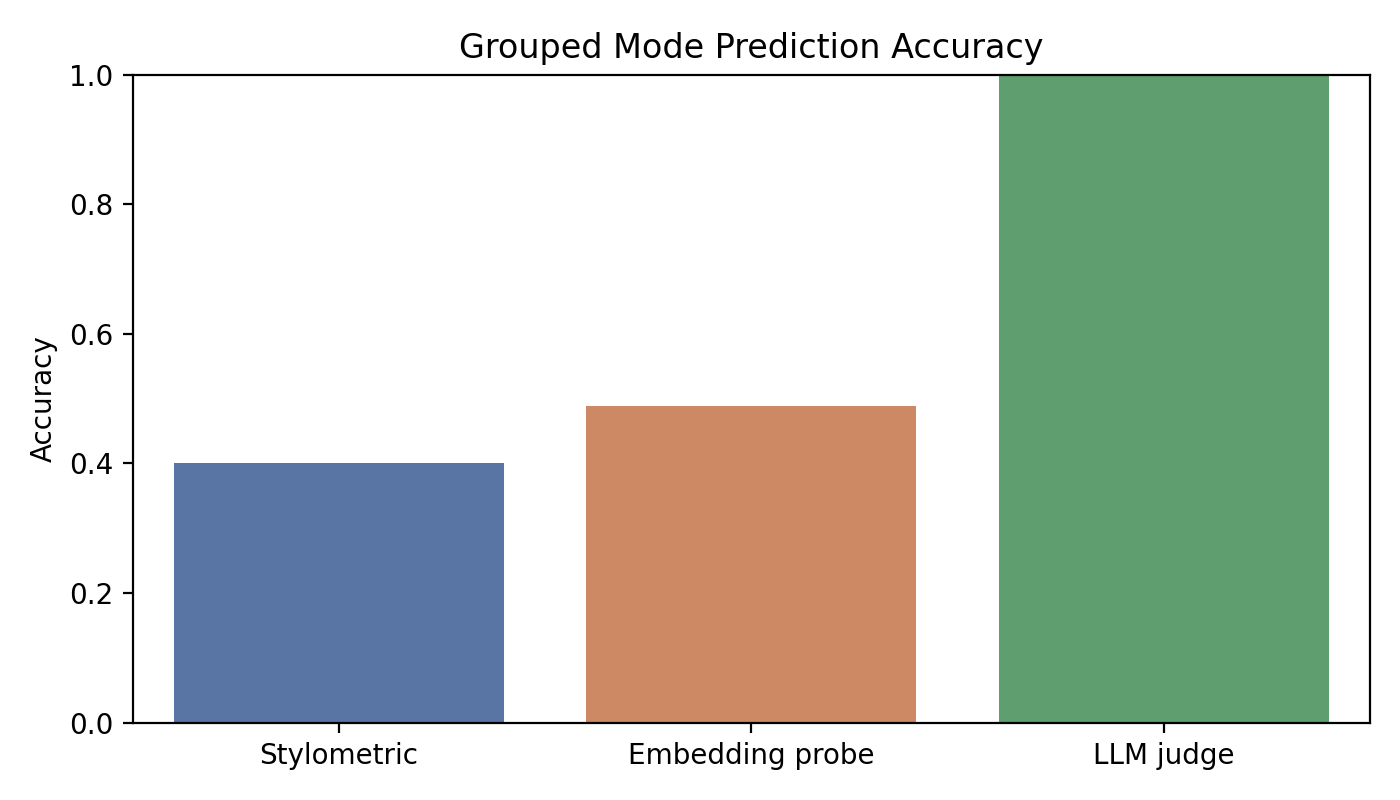
\includegraphics[width=0.72\linewidth]{figures/mode_probe_accuracy.png}
    \caption{Grouped embedding-probe accuracy against the shuffled-label null distribution. The observed score of 0.489 sits well above the null range, which supports the claim that mode information survives content-grouped evaluation.}
    \label{fig:probe_accuracy}
\end{figure}

\para{Mode deltas are directionally consistent.} \Tabref{tab:delta_similarity} summarizes the transformation-vector analysis. All five transformed modes show higher within-mode cosine similarity than between-mode similarity after Benjamini-Hochberg correction. The largest effects occur for \texttt{keyboard\_noisy} and \texttt{dictated\_spoken}, while \texttt{human\_polished} is statistically significant but much weaker.

\begin{table}[t]
    \centering
    \caption{Transformation-vector consistency for each mode. We compare cosine similarity among deltas from \texttt{human\_original} to a transformed variant. Higher within-mode than between-mode similarity supports a reusable mode direction.}
    \label{tab:delta_similarity}
    \begin{tabular}{@{}lccc@{}}
        \toprule
        Mode & Within mean & Between mean & BH-adjusted $p$ \\
        \midrule
        \texttt{keyboard\_noisy} & \textbf{0.111} & -0.015 & $< 10^{-121}$ \\
        \texttt{dictated\_spoken} & 0.094 & 0.027 & $< 10^{-60}$ \\
        \texttt{llm\_humanized} & 0.058 & 0.034 & $4.13 \times 10^{-13}$ \\
        \texttt{llm\_generated} & 0.036 & 0.014 & $6.67 \times 10^{-9}$ \\
        \texttt{human\_polished} & 0.029 & 0.021 & $6.40 \times 10^{-3}$ \\
        \bottomrule
    \end{tabular}
\end{table}


\begin{figure}[t]
    \centering
    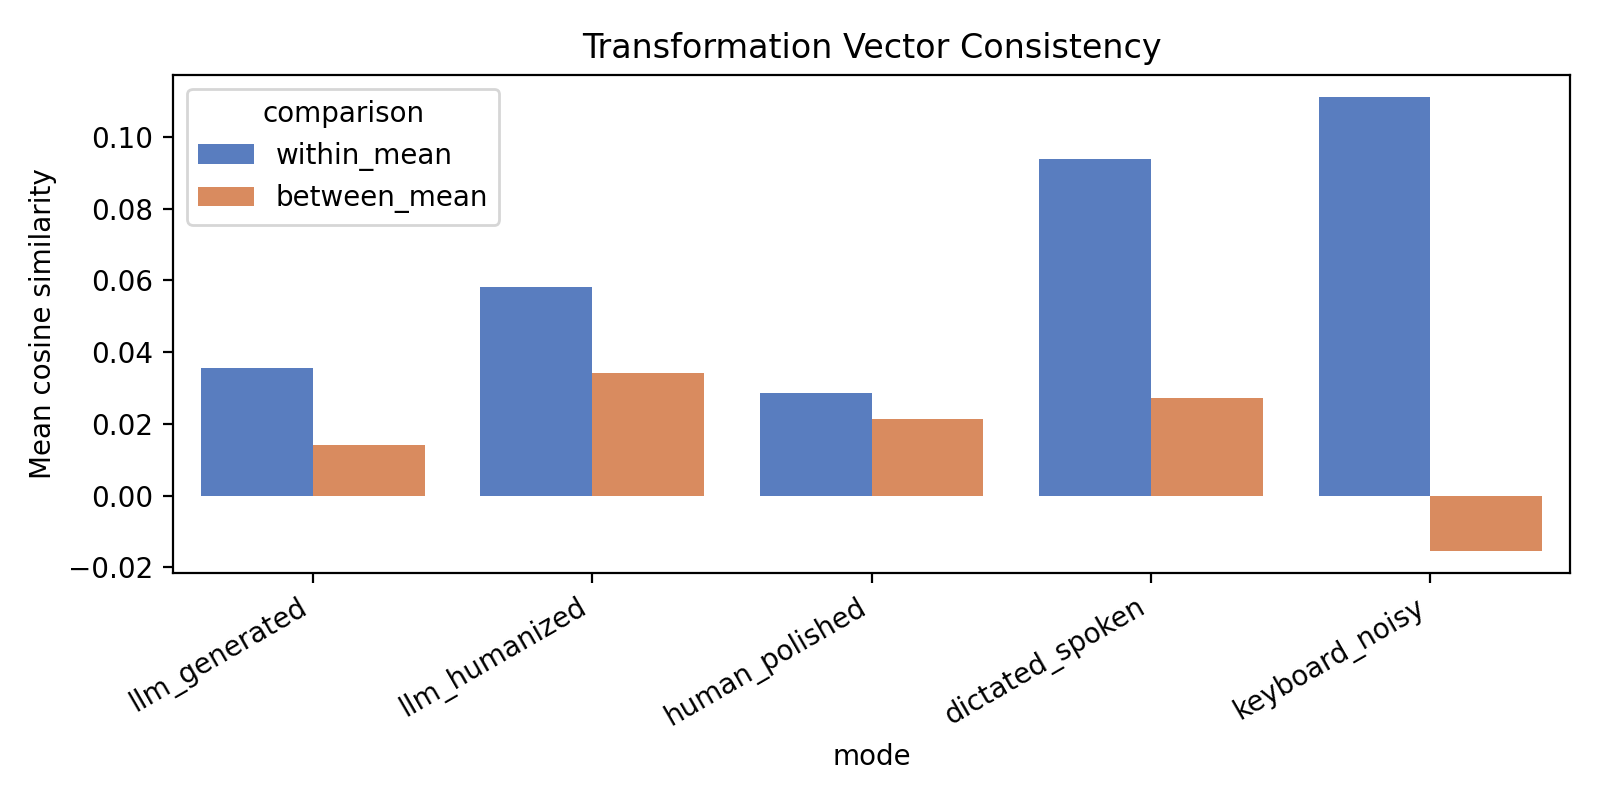
\includegraphics[width=0.78\linewidth]{figures/delta_similarity.png}
    \caption{Within-mode versus between-mode cosine similarity for embedding deltas from \texttt{human\_original} to transformed variants. Larger gaps indicate more reusable mode-specific directions. Keyboard noise and dictated speech produce the clearest latent shifts.}
    \label{fig:delta_similarity}
\end{figure}

\para{External validation sharply narrows the claim.} Strong in-domain mode recognition does not translate into robust zero-shot source attribution. \Tabref{tab:semeval_results} shows that \gptfourone reaches only 0.256 accuracy and 0.136 macro-F1 on \semeval Subtask B, only modestly above the 0.167 chance rate. The bootstrap 95\% confidence interval for accuracy is [0.194, 0.311]. \Figref{fig:semeval_confusion} shows why: the model correctly identifies 29/30 human examples and 17/30 ChatGPT examples, but it collapses almost all Cohere, Davinci, Bloomz, and Dolly examples into the human or ChatGPT labels.

\begin{table}[t]
    \centering
    \caption{External zero-shot source attribution on \semeval Subtask B. Chance accuracy is 0.167. The confidence intervals come from bootstrap resampling.}
    \label{tab:semeval_results}
    \begin{tabular}{@{}lcc@{}}
        \toprule
        Metric & Score & 95\% CI \\
        \midrule
        Accuracy & 0.256 & [0.194, 0.311] \\
        Macro-F1 & 0.136 & [0.108, 0.164] \\
        \bottomrule
    \end{tabular}
\end{table}


\begin{figure}[t]
    \centering
    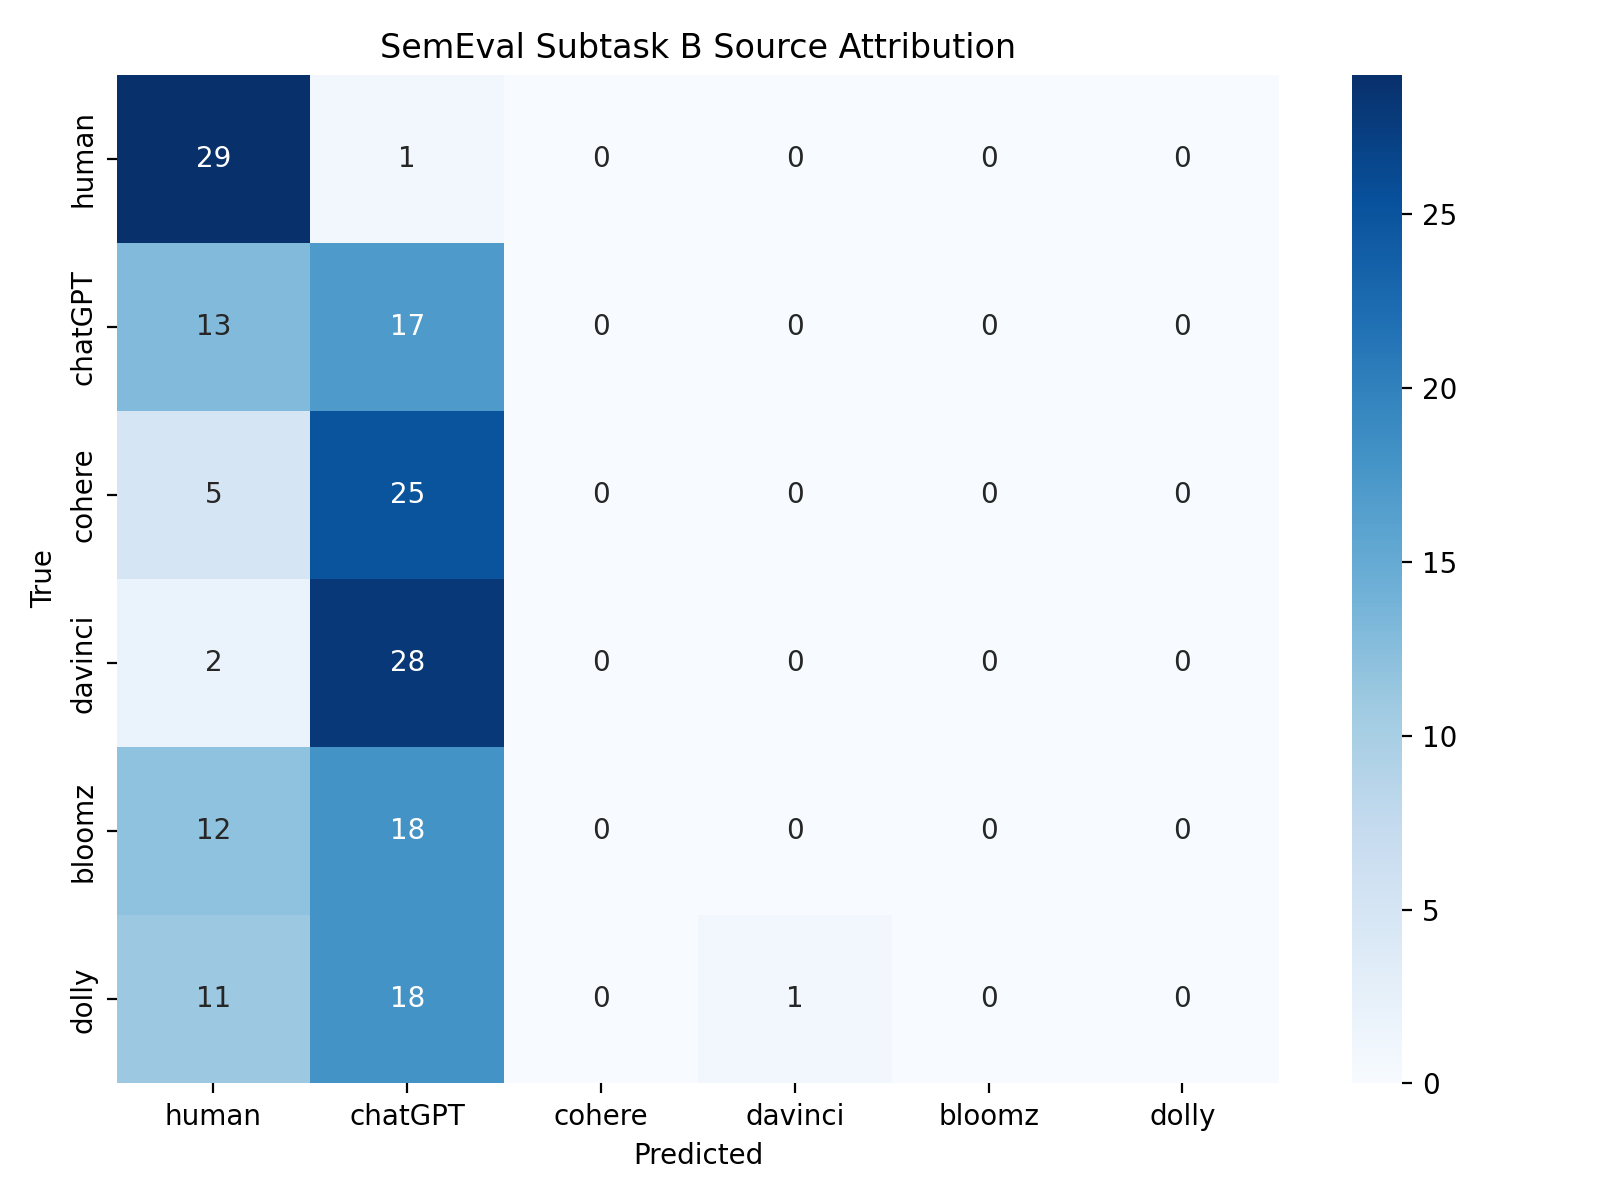
\includegraphics[width=0.78\linewidth]{figures/semeval_subtaskB_confusion.png}
    \caption{Confusion matrix for zero-shot six-way source attribution on \semeval Subtask B. Most non-human systems collapse into \chatgptlabel or human, which indicates that broad process cues transfer more readily than exact generator identity.}
    \label{fig:semeval_confusion}
\end{figure}

\para{What pattern emerges across analyses?} The results consistently point to a hierarchy of detectable modes. Overt production changes such as keyboard noise and spoken-style dictation are strongest in both direct classification and latent-space consistency. Post-editing modes remain detectable, but they are weaker both in per-class probe recall and in delta alignment. Exact zero-shot source identity is weaker still. This ordering is the core empirical claim of the paper.
